%%%%%%%%%%%%%%%%%%%%%%%%%%%%%%%%%%%%%%%%%
% Short Sectioned Assignment
% LaTeX Template
% Version 1.0 (5/5/12)
%
% This template has been downloaded from:
% http://www.LaTeXTemplates.com
%
% Original author:
% Frits Wenneker (http://www.howtotex.com)
%
% License:
% CC BY-NC-SA 3.0 (http://creativecommons.org/licenses/by-nc-sa/3.0/)
%
%%%%%%%%%%%%%%%%%%%%%%%%%%%%%%%%%%%%%%%%%

%----------------------------------------------------------------------------------------
%	PACKAGES AND OTHER DOCUMENT CONFIGURATIONS
%----------------------------------------------------------------------------------------

\documentclass[paper=a4, fontsize=11pt]{article} % A4 paper and 11pt font size

\usepackage[T1]{fontenc} % Use 8-bit encoding that has 256 glyphs
%\usepackage{fourier} % Use the Adobe Utopia font for the document - comment this line to return to the LaTeX default
\usepackage[english]{babel} % English language/hyphenation
\usepackage{amsmath,amsfonts,amsthm} % Math packages
\usepackage[top=2cm, bottom=2cm, right=3cm, left=3cm]{geometry}
\usepackage{lipsum} % Used for inserting dummy 'Lorem ipsum' 1text into the template

\usepackage{sectsty} % Allows customizing section commands
\allsectionsfont{\normalfont} % Make all sections centered, the default font and small caps
\usepackage{cancel}


\usepackage{fancyhdr} % Custom headers and footers
\pagestyle{fancyplain} % Makes all pages in the document conform to the custom headers and footers
\fancyhead{} % No page header - if you want one, create it in the same way as the footers below
\fancyfoot[L]{} % Empty left footer
\fancyfoot[C]{} % Empty center footer
\fancyfoot[R]{\thepage} % Page numbering for right footer
\renewcommand{\headrulewidth}{0pt} % Remove header underlines
\renewcommand{\footrulewidth}{0pt} % Remove footer underlines
\setlength{\headheight}{1pt} % Customize the height of the header

\numberwithin{equation}{section} % Number equations within sections (i.e. 1.1, 1.2, 2.1, 2.2 instead of 1, 2, 3, 4)
\numberwithin{figure}{section} % Number figures within sections (i.e. 1.1, 1.2, 2.1, 2.2 instead of 1, 2, 3, 4)
\numberwithin{table}{section} % Number tables within sections (i.e. 1.1, 1.2, 2.1, 2.2 instead of 1, 2, 3, 4)

\setlength\parindent{0pt} % Removes all indentation from paragraphs - comment this line for an assignment with lots of text

\usepackage{graphicx}
\graphicspath{ {images/} }
\usepackage{hyperref}

%----------------------------------------------------------------------------------------
%	TITLE SECTION
%----------------------------------------------------------------------------------------

\newcommand{\horrule}[1]{\rule{\linewidth}{#1}} % Create horizontal rule command with 1 argument of height

\title{	
\normalfont \normalsize 
\textsc{Polytechnic University of Catalonia} \\ [10pt]
\textsc{\small{ Msc. in Numerical Methods }} \\ [25pt]
\horrule{0.3pt} \\[0.2cm] % Thin top horizontal rule
\LARGE  \textbf{Programming for Engineering and Science} \\ Homework 1: "Matlab and FE" \\ % The assignment title
\horrule{0.3pt} \\[0.1cm] % Thick bottom horizontal rule
}

\author{Albert Capalvo and Lisandro Roldan} % Your name

\date{\normalsize\today} % Today's date or a custom date

\begin{document}

\maketitle

\section{\textbf{Introduction}}

A Matlab program for solving temperature diffusion problems was developed. Some incomplete code was provided by the professors for the solution of a 2D problem using quadrilateral linear elements. That code was modified and extended in order to solve the same problem with different 2D and 3D finite elements and exporting its results for visualization using Paraview.

\section{\textbf{Code description}}

The whole set of Matlab files can be downloaded from the following GitHub repository: \\
\url{<https://github.com/lisandroroldan/FEM2>}\\
The principal program consists on a main file, several functions and input data. All of them can be found in the folder \textit{SS\_ General}.\\
Additionally folders \textit{SS\_ GiD} and \textit{FEM.gid} contain the finite element program and GiD Problem type that was used to generate additional meshes and reference results.

\subsection{\textbf{Main program - part 1}}
\textit{File: main.m}\\

When executed, the user will find a message on the console asking for the name of the problem to be solved. 

Using the load function, the problem's geometry (node location and connectivity matrices ) and groups that define the boundary conditions are imported from data files and converted into Matlab variables.

Automatically, the program will identify the element type to be used. The following types of elements are allowed:\\

2D Elements
\begin{itemize}
\item Triangular linear (3 nodes)
\item Triangular quadratic (6 nodes)
\item Quadrilateral linear (4 nodes)
\item Quadrilateral quadratic (8 nodes)
\end{itemize}
3D Elements
\begin{itemize}
\item Tetrahedral linear (4 nodes)
\item Tetrahedral quadratic (8 nodes)
\item Hexaedron linear (8 nodes)
\item Hexaedron quadratic (20 nodes)
\end{itemize}

From then on, the code will implemented will vary depending on the number of dimensions of the problems and the element type selected. 

The code executes several functions in order to solve the Finite Element problem, witch will be explained bellow.

\subsection{\textbf{Calculation of number of integration points}}
\textit{File: numberofintegrationpoints.m}\\

This function uses the known number of dimensions and amount of nodes per element to return the number of Gauss quadrature integration points to be used.

\subsection{\textbf{Position of Gauss points in normalized coordinate system and integration weights}}
\textit{Files: integrationpoints.m / integrationweights.m}\\

With the same input variables than the last function plus the number of Gauss points, this functions returns a matrix with the standard coordinates for the element in the normalized space and a vector with the weights needed to perform the integration using Gauss quadrature.

\subsection{\textbf{Shape functions and their derivatives}}
\textit{File: shapefunctions.m / shapefunctionderivs.m }\\

Both functions are run inside a loop over the number if integration points, and their outputs are stored in two matrices.

The input for both are the number of dimensions of the problem, the amount of integration points and their position in the normalized space.

The functions choose over many predefined equations to return the desired shape functions and shape functions derivatives with respect to the space coordinates.

\subsection{\textbf{System resulting of discretizing the weak form}}
\textit{Files: CreateMatrix.m / MatEl.m / Isopar.m }\\

This group of nested functions take the node coordinates, connectivity matrix, space dimensions, gauss integration parameters, shape functions and their derivatives to calculate the components of the system of equations to be solved. 

The functions "MatEl" and "Isopar", make the transformation from the normalized space to the real one and create the local stiffness matrices and force vectors (in this case the source term is zero, but it can import the information from a data file). The function "CreateMatrix" ensembles them to get the global system of equations.



\subsection{\textbf{Main program - part 2}}
\textit{File: main.m }\\

Once the global stiffness matrix, force vector and boundary conditions are obtained, the system is solved using the "Lagrange Multipliers Method".

Finally, with the known value of the temperature for every node, a postprocess function is called.

\subsection{\textbf{Post-process}}
\textit{File: postprocess.m }\\

This function creates a .vtk file with a structure and format that is readable by Paraview. Once again, the form and information of the file will vary depending on the element type selected at the beginning.
The output result is a file that contains information about the coordinates of the nodes, their connectivity, the element types used and the solution of the problem.

\section{\textbf{How of use the program}}

When the main file is executed, the user will have to introduce via console the name of the problem to solve:

\begin{center}
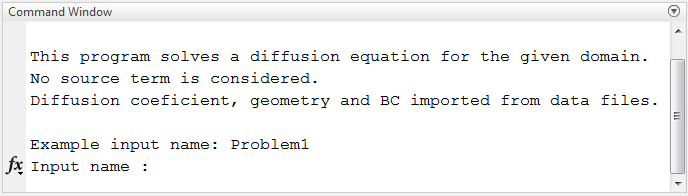
\includegraphics[scale=.75]{input}\\
\textit{Input of problem name}
\end{center}

In case that a different problems with  different geometries than the provided ones are needed to be solved, the user will have to copy the input files into de model and element folder. Their name should have the structure: \textit{Name\_ nodes}, \textit{Name\_ groups}, \textit{Name\_ elements} and \textit{Name\_ prop}.\\

Once the program has finished execution, the user will be asked to input the name of the output file

\begin{center}
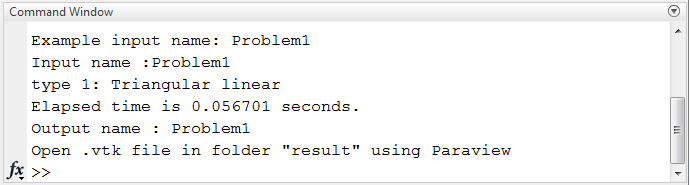
\includegraphics[scale=.75]{output}\\
\textit{Output file name}
\end{center}

The type of element used and the time used for the solving of the problem is informed.

\section{\textbf{Testing and comparison}}

To test the code, all of the eight meshes and groups provided by the professors were used as inputs with the same boundary conditions.

\begin{center}
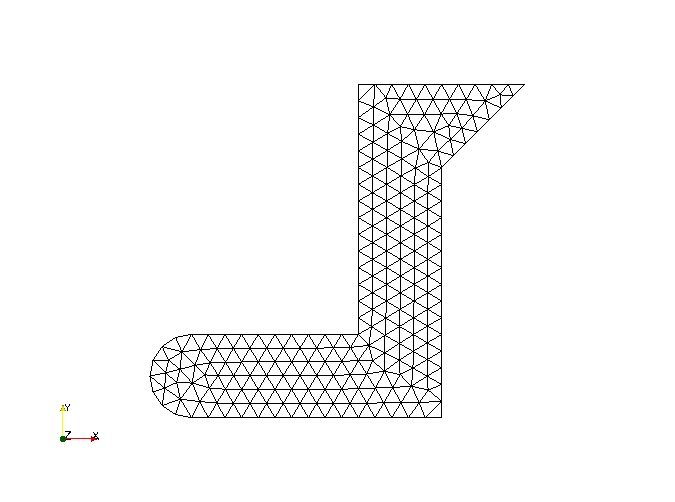
\includegraphics[scale=0.3]{mesh_tri}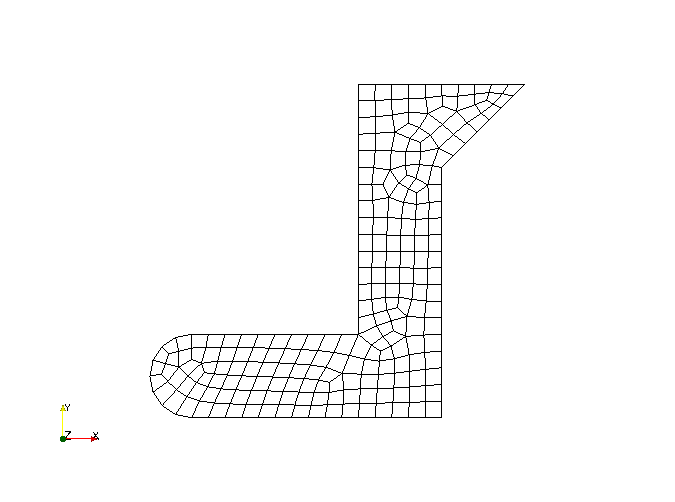
\includegraphics[scale=0.3]{mesh_quad}
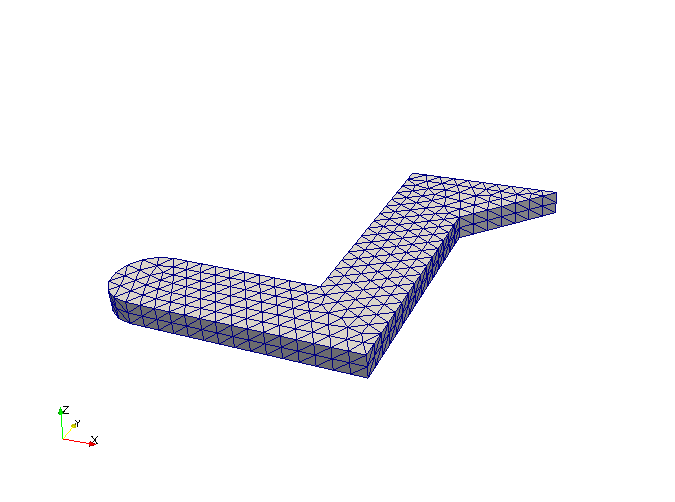
\includegraphics[scale=0.3]{mesh_tet}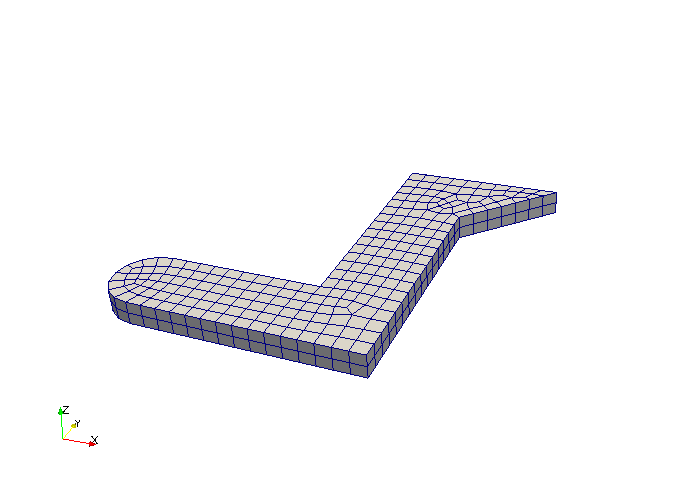
\includegraphics[scale=0.3]{mesh_hexa}

\textit{Top-left: 2D triangular mesh (linear and quadratic); Top-right: 2D quadrilateral mesh (linear and quadratic); Bottom-left: 3D tetrahedral mesh (linear and quadratic); Bottom-right: 3D hexaedral mesh (linear and quadratic).}
\end{center}

Although graphic results were obtained for all of the meshes, no difference can be appreciated graphically, therefore only two examples are included. 

\begin{center}
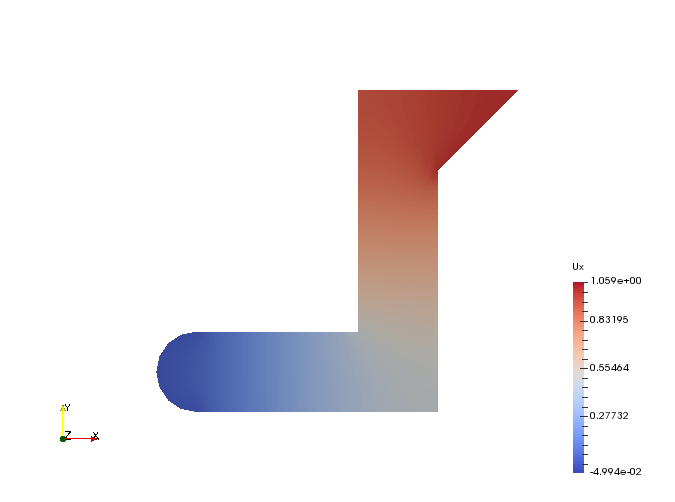
\includegraphics[scale=0.3]{results_2d}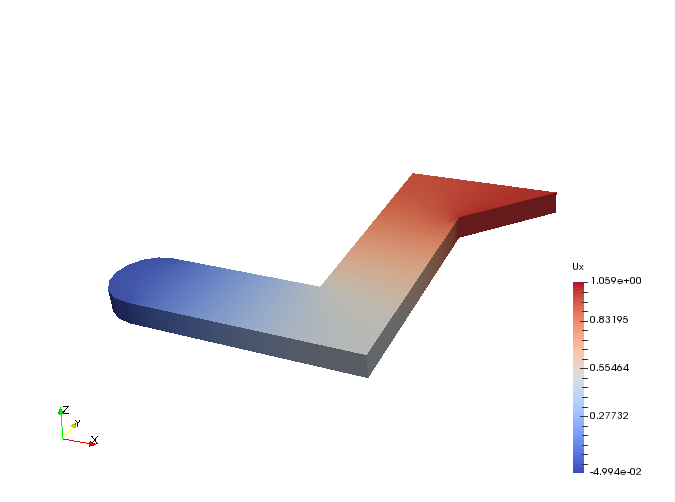
\includegraphics[scale=0.3]{results_3d}


\textit{Left: results for 2D quadratic linear elements; Right: results for 3D hexaedral linear elements}
\end{center}

Using the function tic-toc of Matlab, the execution time was evaluated, producing the following results:
\begin{center}
\begin{tabular}{|c c|c c|}
\hline 
2D\_ TRI\_ LIN & 0.056 sec & 3D\_ TET\_ LIN & 0.516 sec \\ 
\hline 
2D\_ TRI\_ QUAD & 0.149 sec & 3D\_ TET\_ QUAD & 4.308 sec \\ 
\hline 
2D\_ QUAD\_ LIN & 0.068 sec & 3D\_ HEXA\_ LIN & 0.355 sec \\ 
\hline 
2D\_ QUAD\_ QUAD & 0.189 sec & 3D\_ HEXA\_ QUAD & 1.941 sec \\ 
\hline 
\end{tabular} 

\textit{Calculation time}
\end{center}

To compare the results, the another mesh, much denser that the evaluated ones was used as reference, and the relative error was obtained.

Taking advantages that Paraview is able to interpolate the results from the given node values, three points were used to compare results:

\begin{center}
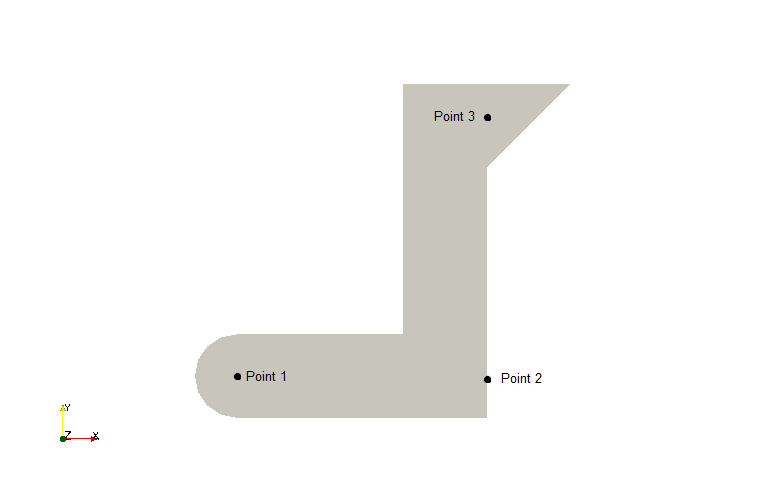
\includegraphics[scale=0.7]{points}

\textit{Points used for comparison}
\end{center}

They were chosen in those positions to see the effect that the shape of the boundary produces on the result precision.\\

\begin{table}[]
\centering
\caption{Relative errors, reference mesh: 48.744 tetrahedral linear elements}
\label{my-label}
\begin{tabular}{|cc|cc|cc|cc|}
\hline
Problem & Type         & \multicolumn{2}{c|}{Point 1 (-25,5)} & \multicolumn{2}{c|}{Point 2 (-5,5)} & \multicolumn{2}{c|}{Point 3 (-5,25)} \\ \hline
Ref     & 3D tet lin   & 0,04499       & Relative error       & 0,48364       & Relative error      & 0,96662       & Relative error       \\
1       & 2D tri lin   & 0,04146       & 7,83\%               & 0,48607       & 0,50\%              & 0,96950       & 0,30\%               \\
2       & 2D tri quad  & 0,04569       & 1,56\%               & 0,48097       & 0,55\%              & 0,96478       & 0,19\%               \\
3       & 2D quad lin  & 0,04333       & 3,68\%               & 0,48393       & 0,06\%              & 0,96756       & 0,10\%               \\
4       & 2D quad quad & 0,04489       & 0,21\%               & 0,48185       & 0,37\%              & 0,96562       & 0,10\%               \\
5       & 3D tet lin   & 0,04170       & 7,31\%               & 0,48624       & 0,54\%              & 0,96960       & 0,31\%               \\
6       & 3D tet quad  & 0,04375       & 2,74\%               & 0,48497       & 0,27\%              & 0,96797       & 0,14\%               \\
7       & 3D hex lin   & 0,04506       & 0,17\%               & 0,48235       & 0,27\%              & 0,96584       & 0,08\%               \\
8       & 3D hex quad  & 0,04501       & 0,04\%               & 0,48266       & 0,20\%              & 0,96613       & 0,05\%               \\ \hline
\end{tabular}
\end{table}

It can be observed that the results have bigger error when a point near the curved boundary is evaluated. Specially linear triangles and tetrahedral elements present important differences as the values of the temperature are lower than the reference.

\section{\textbf{Challenges encountered}}

There were several challenges to be sorted. First, the understanding of the basic algorithm for a simple case of rectangular 2D geometry with linear rectangular elements.\\

Then, extending the program to work also in 3D and all of the element types described bellow.
It is important to remark that the original files had errors in the functions \textit{shapefunctions.m} and \textit{shapefunctionsderiv.m}, which lead to incoherent results. Their identification and corrections took most of the time.\\

Finally, a GiD problem type was developed. A new model with the same geometry was created and a denser mesh was obtained to be used to obtain the a reference to calculate the relative error of the given geometries.

\section{\textbf{Conclusions}}





\end{document}



